\clearpage
\section{Messung} % (fold)
\label{sec:messung}

Zunächst wird die Stärke des gesamten Horizontalfeldes in Abhängigkeit von der Resonanzfrequenz für die Isotope bestimmt.
Anschließend wird das Isotopenverhältnis aus den beobachteten Amplituden berechnet, wodurch eine Zuordnung möglich ist.
Weiterhin wird die Horizontalfeldkomponente des lokalen Erdmagnetfeldes und die Landéschen g$_\text{F}$-Faktoren der Isotope berechnet, woraus wiederum die zugehöigen Kernspins bestimmt werden.
Abschließend kann die größe des quadratischen Zeeman-Effektes abgeschätzt und die Perioden der Schwingung untersucht werden.
Zur Berechnung der Fehler wurde die uncertainties Bibliothek in python genutzt, wodurch der Fehler nach
\begin{equation*}
    \Delta f = \sqrt{\sum_{i=1}^N \left( \left(\frac{\partial f}{\partial x_i}\right)^2  \Delta f_{x_i}^2 \right)}
\end{equation*}
berechnet wird \cite{py-uncertainties}.

\subsection{Berechnung des Isotopenverhältnisses} % (fold)
\label{sub:berechnung_des_isotopenver}

Abbildung \ref{fig:typisches_signalbild} zeigt ein typisches Signalbild der Messung.
Aus den Absorptionsamplituden $A_i$ der Rubidium Isotope lässt sich mithilfe der Gleichungen
\begin{align*}
    X \cdot \text{Rb}_1 + Y \cdot \text{Rb}_2 &= \text{Rb}_\text{Probe}\,,\\
    X + Y &= 1\,,\\
    Y &= \left(1 + \frac{X}{Y} \right)^{-1}\,,\\
    \frac{X}{Y} &= \frac{A_1}{A_2}\,,
\end{align*}
das Isotopenverhältnis berechnen.
Aus der Abbildung kann $A_1$ zu $(\input{build/tex/c_ratio_87.tex})\,$a.u. und $A_2$ zu $(\input{build/tex/c_ratio_85.tex})\,$a.u. bestimmt werden und es ergeben sich die in Tabelle \ref{tab:magnet_data_ratio} dargestellten prozentualen Anteile.
Somit kann der erste Peak dem Isotop Rubidium 87 und der zweite Peak dem Isotop Rubidium 85 zugeordnet werden.

\begin{table}[!h]
    \centering
    \caption{Isotopenverhältnis von Rubidium 85 und Rubidium 87 in der untersuchten Probe.}
    \begin{tabular}{S[table-format=2.1(1)] S[table-format=2.1(1)]}
\toprule
\multicolumn{1}{c}{#Rb$_\text{87} / \si{\percent}$} & \multicolumn{1}{c}{#Rb$_\text{85} / \si{\percent}$}\\
\midrule
35.3 \pm 2.2 & 64.7 \pm 2.2 \\
\bottomrule
\end{tabular}
    \label{tab:magnet_data_ratio}
\end{table}

\begin{figure}[!h]
    \centering
    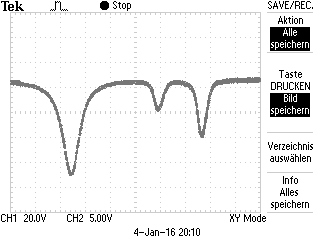
\includegraphics[width=0.7\linewidth]{data/TEK0002.jpg}
    \caption{Typisches Signalbild der Messung. Auf der X-Achse ist die stärke des horizontalen Magnetfeldes und auf der Y-Achse der detektierte Photonenstrom dargestellt.}
    \label{fig:typisches_signalbild}
\end{figure}

\FloatBarrier
\subsection{Messung des Horizontalfeldes} % (fold)
\label{sub:typisches_signalbild}

Zur Messung des gesamten Horizontalfeldes bei induzierter Emission wird mithilfe der Horizontalfeldspule und der Sweepspule die Resonanzstelle eingestellt.
Die benötigten Spulenströme sind in Tabelle \ref{tab:magnet_data_raw} dargestellt.
Mithilfe der Daten der Spulen
\begin{align*}
    R_\text{Sweep} &= \SI{16.39}{\centi\meter}\,,\\
    N_\text{Sweep} &= \SI{11}{Windungen}\,,\\
    R_\text{Hor} &= \SI{15.79}{\centi\meter}\,,\\
    N_\text{Hor} &= \SI{154}{Windungen}\,,
\end{align*}
und der Helmholtzformel
\begin{align*}
    B(0) &= \frac{\mu_0 8 I N}{\sqrt{125} R}\,,
\end{align*}
ergeben sich die zugehörigen Magnetfelder, welche in Tabelle \ref{tab:magnet_gesamt} dargestellt sind.

\begin{table}[!h]
    \centering
    \caption{Werte des Spulenstromes in Abhängigkeit von der Resonanzfrequenz an der Resonanzstelle.}
    \begin{tabular}{S[table-format=4.4(4)] S[table-format=3.1(1)] S[table-format=2.1(1)]}
\toprule
\multicolumn{1}{c}{$\nu / \si{\kilo\hertz}$} & \multicolumn{1}{c}{$I_\text{0,sweep} / \si{\milli\ampere}$} & \multicolumn{1}{c}{$I_\text{0,hor} / \si{\milli\ampere}$}\\
\midrule
100.0000 \pm 0.0005 & 295.0 \pm 0.5 & 0.0 \pm 0.5 \\
200.0000 \pm 0.0005 & 127.0 \pm 0.5 & 5.0 \pm 0.5 \\
300.0000 \pm 0.0005 & 290.0 \pm 0.5 & 0.0 \pm 0.5 \\
400.0000 \pm 0.0005 & 300.0 \pm 0.5 & 0.0 \pm 0.5 \\
500.0000 \pm 0.0005 & 303.0 \pm 0.5 & 0.0 \pm 0.5 \\
600.0000 \pm 0.0005 & 291.0 \pm 0.5 & 0.0 \pm 0.5 \\
700.0000 \pm 0.0005 & 300.0 \pm 0.5 & 0.0 \pm 0.5 \\
800.0000 \pm 0.0005 & 300.0 \pm 0.5 & 0.0 \pm 0.5 \\
900.0000 \pm 0.0005 & 300.0 \pm 0.5 & 0.0 \pm 0.5 \\
1000.0000 \pm 0.0005 & 297.0 \pm 0.5 & 0.0 \pm 0.5 \\
\midrule
\multicolumn{1}{c}{$\nu / \si{\kilo\hertz}$} & \multicolumn{1}{c}{$I_\text{87,sweep} / \si{\milli\ampere}$} & \multicolumn{1}{c}{$I_\text{87,hor} / \si{\milli\ampere}$}\\
\midrule
100.0000 \pm 0.0005 & 534.0 \pm 0.5 & 0.0 \pm 0.5 \\
200.0000 \pm 0.0005 & 604.0 \pm 0.5 & 5.0 \pm 0.5 \\
300.0000 \pm 0.0005 & 462.0 \pm 0.5 & 13.0 \pm 0.5 \\
400.0000 \pm 0.0005 & 404.0 \pm 0.5 & 20.0 \pm 0.5 \\
500.0000 \pm 0.0005 & 154.0 \pm 0.5 & 31.0 \pm 0.5 \\
600.0000 \pm 0.0005 & 236.0 \pm 0.5 & 34.0 \pm 0.5 \\
700.0000 \pm 0.0005 & 69.0 \pm 0.5 & 44.0 \pm 0.5 \\
800.0000 \pm 0.0005 & 406.0 \pm 0.5 & 41.0 \pm 0.5 \\
900.0000 \pm 0.0005 & 452.0 \pm 0.5 & 46.0 \pm 0.5 \\
1000.0000 \pm 0.0005 & 564.0 \pm 0.5 & 49.0 \pm 0.5 \\
\midrule
\multicolumn{1}{c}{$\nu / \si{\kilo\hertz}$} & \multicolumn{1}{c}{$I_\text{85,sweep} / \si{\milli\ampere}$} & \multicolumn{1}{c}{$I_\text{85,hor} / \si{\milli\ampere}$}\\
\midrule
100.0000 \pm 0.0005 & 653.0 \pm 0.5 & 0.0 \pm 0.5 \\
200.0000 \pm 0.0005 & 839.0 \pm 0.5 & 5.0 \pm 0.5 \\
300.0000 \pm 0.0005 & 816.0 \pm 0.5 & 13.0 \pm 0.5 \\
400.0000 \pm 0.0005 & 816.0 \pm 0.5 & 20.0 \pm 0.5 \\
500.0000 \pm 0.0005 & 732.0 \pm 0.5 & 31.0 \pm 0.5 \\
600.0000 \pm 0.0005 & 944.0 \pm 0.5 & 34.0 \pm 0.5 \\
700.0000 \pm 0.0005 & 899.0 \pm 0.5 & 44.0 \pm 0.5 \\
800.0000 \pm 0.0005 & 745.0 \pm 0.5 & 56.0 \pm 0.5 \\
900.0000 \pm 0.0005 & 718.0 \pm 0.5 & 64.0 \pm 0.5 \\
1000.0000 \pm 0.0005 & 790.0 \pm 0.5 & 71.0 \pm 0.5 \\
\bottomrule
\end{tabular}

    \label{tab:magnet_data_raw}
\end{table}

\begin{table}[!h]
    \centering
    \caption{Werte des gesamten Horizontalfeldes in Abhängigkeit von der Resonanzfrequenz an der Resonanzstelle.}
    \begin{tabular}{S[table-format=4.4(4)] S[table-format=3.1(1)] S[table-format=3.1(1)] S[table-format=2.3(3)]}
\toprule
\multicolumn{1}{c}{$\nu / \si{\kilo\hertz}$} & \multicolumn{1}{c}{$B_\text{0,ges} / \si{\micro\tesla}$} & \multicolumn{1}{c}{$B_\text{0,sweep} / \si{\micro\tesla}$} & \multicolumn{1}{c}{$B_\text{0,hor} / \si{\micro\tesla}$}\\
\midrule
100.0000 \pm 0.0005 & 17.8 \pm 1.3 & 0.0 \pm 1.3 & 17.802 \pm 0.030 \\
200.0000 \pm 0.0005 & 20.8 \pm 1.3 & 13.2 \pm 1.3 & 7.664 \pm 0.030 \\
300.0000 \pm 0.0005 & 17.5 \pm 1.3 & 0.0 \pm 1.3 & 17.501 \pm 0.030 \\
400.0000 \pm 0.0005 & 18.1 \pm 1.3 & 0.0 \pm 1.3 & 18.104 \pm 0.030 \\
500.0000 \pm 0.0005 & 18.3 \pm 1.3 & 0.0 \pm 1.3 & 18.285 \pm 0.030 \\
600.0000 \pm 0.0005 & 17.6 \pm 1.3 & 0.0 \pm 1.3 & 17.561 \pm 0.030 \\
700.0000 \pm 0.0005 & 18.1 \pm 1.3 & 0.0 \pm 1.3 & 18.104 \pm 0.030 \\
800.0000 \pm 0.0005 & 18.1 \pm 1.3 & 0.0 \pm 1.3 & 18.104 \pm 0.030 \\
900.0000 \pm 0.0005 & 18.1 \pm 1.3 & 0.0 \pm 1.3 & 18.104 \pm 0.030 \\
1000.0000 \pm 0.0005 & 17.9 \pm 1.3 & 0.0 \pm 1.3 & 17.923 \pm 0.030 \\
\midrule
\multicolumn{1}{c}{$\nu / \si{\kilo\hertz}$} & \multicolumn{1}{c}{$B_\text{87,ges} / \si{\micro\tesla}$} & \multicolumn{1}{c}{$B_\text{87,sweep} / \si{\micro\tesla}$} & \multicolumn{1}{c}{$B_\text{87,hor} / \si{\micro\tesla}$}\\
\midrule
100.0000 \pm 0.0005 & 32.2 \pm 1.3 & 0.0 \pm 1.3 & 32.226 \pm 0.030 \\
200.0000 \pm 0.0005 & 49.6 \pm 1.3 & 13.2 \pm 1.3 & 36.450 \pm 0.030 \\
300.0000 \pm 0.0005 & 62.1 \pm 1.3 & 34.2 \pm 1.3 & 27.880 \pm 0.030 \\
400.0000 \pm 0.0005 & 77.0 \pm 1.3 & 52.6 \pm 1.3 & 24.380 \pm 0.030 \\
500.0000 \pm 0.0005 & 90.9 \pm 1.3 & 81.6 \pm 1.3 & 9.293 \pm 0.030 \\
600.0000 \pm 0.0005 & 103.7 \pm 1.3 & 89.5 \pm 1.3 & 14.242 \pm 0.030 \\
700.0000 \pm 0.0005 & 119.9 \pm 1.3 & 115.8 \pm 1.3 & 4.164 \pm 0.030 \\
800.0000 \pm 0.0005 & 132.4 \pm 1.3 & 107.9 \pm 1.3 & 24.501 \pm 0.030 \\
900.0000 \pm 0.0005 & 148.3 \pm 1.3 & 121.0 \pm 1.3 & 27.277 \pm 0.030 \\
1000.0000 \pm 0.0005 & 163.0 \pm 1.3 & 128.9 \pm 1.3 & 34.036 \pm 0.030 \\
\midrule
\multicolumn{1}{c}{$\nu / \si{\kilo\hertz}$} & \multicolumn{1}{c}{$B_\text{85,ges} / \si{\micro\tesla}$} & \multicolumn{1}{c}{$B_\text{85,sweep} / \si{\micro\tesla}$} & \multicolumn{1}{c}{$B_\text{85,hor} / \si{\micro\tesla}$}\\
\midrule
100.0000 \pm 0.0005 & 39.4 \pm 1.3 & 0.0 \pm 1.3 & 39.407 \pm 0.030 \\
200.0000 \pm 0.0005 & 63.8 \pm 1.3 & 13.2 \pm 1.3 & 50.631 \pm 0.030 \\
300.0000 \pm 0.0005 & 83.4 \pm 1.3 & 34.2 \pm 1.3 & 49.243 \pm 0.030 \\
400.0000 \pm 0.0005 & 101.9 \pm 1.3 & 52.6 \pm 1.3 & 49.243 \pm 0.030 \\
500.0000 \pm 0.0005 & 125.7 \pm 1.3 & 81.6 \pm 1.3 & 44.174 \pm 0.030 \\
600.0000 \pm 0.0005 & 146.4 \pm 1.3 & 89.5 \pm 1.3 & 56.968 \pm 0.030 \\
700.0000 \pm 0.0005 & 170.0 \pm 1.3 & 115.8 \pm 1.3 & 54.252 \pm 0.030 \\
800.0000 \pm 0.0005 & 192.3 \pm 1.3 & 147.3 \pm 1.3 & 44.959 \pm 0.030 \\
900.0000 \pm 0.0005 & 211.7 \pm 1.3 & 168.4 \pm 1.3 & 43.329 \pm 0.030 \\
1000.0000 \pm 0.0005 & 234.5 \pm 1.3 & 186.8 \pm 1.3 & 47.674 \pm 0.030 \\
\bottomrule
\end{tabular}

    \label{tab:magnet_gesamt}
\end{table}

\FloatBarrier
\subsection{Lokales Erdmagnetfeld} % (fold)
\label{sub:lokales_erdmagnetfeld}

Es lassen sich nun die horizontale und die vertikale Komponente des Erdmagnetfeldes bestimmen.
Die errechneten Werte sind in Tabelle \ref{tab:erd} dargestellt.
Die vertikale Komponente entspricht dem Magnetfeld der Vertikalfeldspule.
Mit den Daten dieser Spule
\begin{align*}
    R_\text{Vert} &= \SI{11.735}{\centi\meter}\,,\\
    N_\text{Vert} &= \SI{20}{Windungen}\,,
\end{align*}
kann der Wert $\input{build/tex/c_vert.tex}$ ermittelt werden.
Das Magnetfeld an der Resonanzstelle $0$, welche keinem der beiden Isotope zugeordnet worden ist, entspricht der horizontalen Komponente.
Da diese Frequenzunabhängig ist, kann sie durch Mittelung bei den verschiedenen Frequenzen ermittelt werden.

\begin{table}[!h]
    \centering
    \caption{Errechnete Komponenten des lokalen Erdmagnetfeldes.}
    \begin{tabular}{S[table-format=2.2(2)] S[table-format=2.1(1)]}
\toprule
\multicolumn{1}{c}{$B_\text{Vert} / \si{\micro\tesla}$} & \multicolumn{1}{c}{$B_\text{Hor} / \si{\micro\tesla}$}\\
\midrule
39.84 \pm 0.08 & 18.2 \pm 0.4 \\
\bottomrule
\end{tabular}
    \label{tab:erd}
\end{table}

\FloatBarrier
\subsection{Landéschen g$_\text{F}$-Faktoren und Kernspin} % (fold)
\label{sub:landeschen_g_text}

Weiterhin lassen sich aus den bestimmten Magnetfeldern die Landéschen g$_\text{F}$-Faktoren der Isotope und daraus der Kernspins bestimmen.
Die errechneten Faktoren sind in Tabelle \ref{tab:lande_faktor} dargestellt.
Zur Berechnung der lässt sich Gleichung \eqref{eq:resonanz} umschreiben zu
\begin{align*}
    B_m &= \frac{4 \pi m_0}{e_0 g_\text{F}} \nu \,.
\end{align*}
Mithilfe einer linearer Regressionen der Form $a(\nu)=m_\text{87} \cdot \nu + b$ und $b(\nu)=m_\text{85} \cdot \nu + b$ ergeben sich für die Isotope
\begin{align*}
    m_{87} &= \SI{1.4306e-10}{\tesla\per\hertz}\,,\\
    b_{87} &= \SI{1.9219e-05}{\tesla\per\hertz}\,,\\
    g_\text{F, 87} &= \frac{4 \pi m_0}{m_{87} e_0}\,,\\
    m_{85} &= \SI{2.1578e-10}{\tesla\per\hertz}\,,\\
    b_{85} &= \SI{1.8234e-05}{\tesla\per\hertz}\,,\\
    g_\text{F, 85} &= \frac{4 \pi m_0}{m_{87} e_0}\,.
\end{align*}
Die zugehörige graphische Darstellung ist in den Abbildungen \ref{fig:fit_lande_87} und \ref{fig:fit_lande_85} dargestellt.
Da die Fehler hinreichend klein sind, wurden diese in der weiteren Rechnung nicht berücksichtigt.

Der Faktor g$_\text{J}$ lässt sich nun für die Isotope mithilfe von Gleichung \ref{eq:gj} berechnen.
Da sich die Isotope nur in ihrem Kernspin unterscheiden, ergibt sich für die Quantenzahlen von Rubidium
\begin{align*}
    S &= \frac{1}{2}\,,\\
    L &= 0\,,\\
    J &= \frac{1}{2}\,.
\end{align*}

Für die Berechnung des Kernspins kann Gleichung \ref{eq:lande_faktor} unter der Berücksichtigung, dass $F = I + J$ gilt, umgestellt werden zu
\begin{align*}
    I &= \frac{4 g_\text{F} - g_\text{J}}{4 g_\text{F}} + \sqrt{\left(\frac{4 g_\text{F} - g_\text{J}}{4 g_\text{F}}\right)^2 - \frac{3}{4}(1 - \frac{g_\text{J}}{g_\text{F}})} \,.
\end{align*}
Somit berechnet sich der Kernspin von Rubidium 87 zu $I = \input{build/tex/c_I_87.tex}$ und von Rubifium 85 zu $I = \input{build/tex/c_I_85.tex}$.

\begin{table}[!h]
    \centering
    \caption{Landéschen g$_\text{F}$-Faktoren und Kernspins der Rubidium Isotop.}
    \begin{tabular}{S[table-format=1.17] S[table-format=1.17] S[table-format=1.4] S[table-format=1.16] S[table-format=1.16]}
\toprule
\multicolumn{1}{c}{$g_\text{f,1} / \si{}$} & \multicolumn{1}{c}{$g_\text{f,2} / \si{}$} & \multicolumn{1}{c}{$g_\text{j} / \si{}$} & \multicolumn{1}{c}{$I_\text{1} / \si{}$} & \multicolumn{1}{c}{$I_\text{2} / \si{}$}\\
\midrule
0.49943830208187645 & 0.33111457925448684 & 2.0023 & 1.5045519052639147 & 2.5235757128366725 \\
\bottomrule
\end{tabular}
    \label{tab:lande_faktor}
\end{table}

\begin{figure}[!h]
    \centering
    \includegraphics[width = 14cm]{build/plots/c_fit_87.pdf}
    \caption{Messwerte und lineare Ausgleichsgerade zur Berechnung des Landéschen g$_\text{F}$-Faktors von Rubidium 87.}
    \label{fig:fit_lande_87}
\end{figure}

\begin{figure}[!h]
    \centering
    \includegraphics[width = 14cm]{build/plots/c_fit_85.pdf}
    \caption{Messwerte und lineare Ausgleichsgerade zur Berechnung des Landéschen g$_\text{F}$-Faktors von Rubidium 85.}
    \label{fig:fit_lande_85}
\end{figure}

\FloatBarrier
\subsection{Abschätzung des quadratischen Zeeman-Effekts} % (fold)
\label{sub:quadratischer_zeeman_effekt}

Die Näherung des Zeeman-Effekts von der Ordnung B$^2$ kann durch den Term 1. Ordnung
\begin{align*}
    U_\text{1.} &= g_F \mu_B B \,,
\end{align*}
und den Term 2. Ordnung
\begin{align*}
    U_\text{2.} &= (g_F\mu_B B)^2 \cdot \frac{1 - 2M_F}{\Delta E_\text{Hy}} \,,
\end{align*}
beschrieben werden.
Da für die Werte der Quantenzahl $M_\text{F}$ ganze Zahlen von $-2$ bis $2$ möglich sind, können die Größenordnungen der Terme 1. und 2. Ordnung bei verschiedenen $M_\text{F}$ miteinander verglichen werden.
Die Ergebnisse für die verschiedenen Isotope sind in den Tabellen \ref{tab:square_87_0} bis \ref{tab:square_85_4} dargestellt.

\begin{table}[!h]
    \centering
    \caption{Ergebnisse der Berechnung des Quadratischen Zeeman-Effekts bei $M_\text{F} = -2$ bei den berechneten Magnetfeldern $B_\text{Ges}$ für Rubidium 87.}
    \input{build/tex/c_data_square_87_0.tex}
    \label{tab:square_87_0}
\end{table}

\begin{table}[!h]
    \centering
    \caption{Ergebnisse der Berechnung des Quadratischen Zeeman-Effekts bei $M_\text{F} = -1$ bei den berechneten Magnetfeldern $B_\text{Ges}$ für Rubidium 87.}
    \input{build/tex/c_data_square_87_1.tex}
    \label{tab:square_87_1}
\end{table}

\begin{table}[!h]
    \centering
    \caption{Ergebnisse der Berechnung des Quadratischen Zeeman-Effekts bei $M_\text{F} = 0$ bei den berechneten Magnetfeldern $B_\text{Ges}$ für Rubidium 87.}
    \input{build/tex/c_data_square_87_2.tex}
    \label{tab:square_87_2}
\end{table}

\begin{table}[!h]
    \centering
    \caption{Ergebnisse der Berechnung des Quadratischen Zeeman-Effekts bei $M_\text{F} = 1$ bei den berechneten Magnetfeldern $B_\text{Ges}$ für Rubidium 87.}
    \input{build/tex/c_data_square_87_3.tex}
    \label{tab:square_87_3}
\end{table}

\begin{table}[!h]
    \centering
    \caption{Ergebnisse der Berechnung des Quadratischen Zeeman-Effekts bei $M_\text{F} = 2$ bei den berechneten Magnetfeldern $B_\text{Ges}$ für Rubidium 87.}
    \input{build/tex/c_data_square_87_4.tex}
    \label{tab:square_87_4}
\end{table}

\begin{table}[!h]
    \centering
    \caption{Ergebnisse der Berechnung des Quadratischen Zeeman-Effekts bei $M_\text{F} = -2$ bei den berechneten Magnetfeldern $B_\text{Ges}$ für Rubidium 85.}
    \input{build/tex/c_data_square_85_0.tex}
    \label{tab:square_85_0}
\end{table}

\begin{table}[!h]
    \centering
    \caption{Ergebnisse der Berechnung des Quadratischen Zeeman-Effekts bei $M_\text{F} = -1$ bei den berechneten Magnetfeldern $B_\text{Ges}$ für Rubidium 85.}
    \input{build/tex/c_data_square_85_1.tex}
    \label{tab:square_85_1}
\end{table}

\begin{table}[!h]
    \centering
    \caption{Ergebnisse der Berechnung des Quadratischen Zeeman-Effekts bei $M_\text{F} = 0$ bei den berechneten Magnetfeldern $B_\text{Ges}$ für Rubidium 85.}
    \input{build/tex/c_data_square_85_2.tex}
    \label{tab:square_85_2}
\end{table}

\begin{table}[!h]
    \centering
    \caption{Ergebnisse der Berechnung des Quadratischen Zeeman-Effekts bei $M_\text{F} = 1$ bei den berechneten Magnetfeldern $B_\text{Ges}$ für Rubidium 85.}
    \input{build/tex/c_data_square_85_3.tex}
    \label{tab:square_85_3}
\end{table}

\begin{table}[!h]
    \centering
    \caption{Ergebnisse der Berechnung des Quadratischen Zeeman-Effekts bei $M_\text{F} = 2$ bei den berechneten Magnetfeldern $B_\text{Ges}$ für Rubidium 85.}
    \input{build/tex/c_data_square_85_4.tex}
    \label{tab:square_85_4}
\end{table}

\FloatBarrier
\subsection{Untersuchung der Perioden der Oszillation} % (fold)
\label{sub:subsection_name}

Bei der untersuchung der Perioden der Oszillation für die Rubidium Isotope 85 und 87 wird zunächst die ansteigende Flanke untersucht und anschließend die Perioden als Funktion der RF-Modulation.

\subsubsection{Exponentialfunktion der ansteigenden Flanke} % (fold)
\label{ssub:exponentialfunktion_der_ansteigenden_flanke}

Bei der Berechnung liegen die Daten der Abbildungen \ref{fig:exp_87_raw} und \ref{fig:exp_85_raw} der RF-Modulation der Isotope zugrunde.
Diese sind graphisch in den Abbildungen \ref{fig:exp_87} und \ref{fig:exp_85} dargestellt.
Zur Berechnung der Exponentialkoeffizienten $\tau$ werden die Messdaten logarithmiert und anschließend mithilfe einer linearen Regression der Form $c(t)=m_\text{87} \cdot t + b$ und $d(t)=m_\text{85} \cdot t + b$ diese als deren negative Steigung $-m$ bestimmt.
Um eine offsetfreie Exponentialfunktion zu logarithmieren, werden die hinteren Bereiche der Funktionen gemittelt und zu Off$_\text{87} = \input{build/tex/i_average_87.tex}$ und Off$_\text{85} = \input{build/tex/i_average_85.tex}$ bestimmt.
Anschließend werden die Offsetwerte von den Messwerten substrahiert und in dem linearen Bereich der logarithmierten Werte die Steigung bestimmt.
Der Anstieg der Anstiegskurve ist auf die Bereiche
\begin{align*}
    t_\text{0, 87} &= \input{build/tex/i_fit_start_87.tex} \,,\\
    t_\text{1, 87} &= \input{build/tex/i_fit_end_87.tex} \,,\\
    t_\text{0, 85} &= \input{build/tex/i_fit_start_85.tex} \,,\\
    t_\text{1, 85} &= \input{build/tex/i_fit_end_85.tex} \,,
\end{align*}
abgeschätzt worden.
Die linearen Regressionen und somit die Exponentialkoeffizienten $\tau$ ergeben sich zu
\begin{align*}
    m_\text{87} &= \input{build/tex/i_fit_m_87.tex} \,,\\
    b_\text{87} &= \input{build/tex/i_fit_b_87.tex} \,,\\
    \tau_\text{87} &= \input{build/tex/i_fit_tau_87.tex} \,,\\
    m_\text{85} &= \input{build/tex/i_fit_m_85.tex} \,,\\
    b_\text{85} &= \input{build/tex/i_fit_b_85.tex} \,.\\
    \tau_\text{87} &= \input{build/tex/i_fit_tau_87.tex} \,,
\end{align*}
Nicht angegebene Fehler sind nicht signifikant.

\begin{figure}[!h]
    \centering
    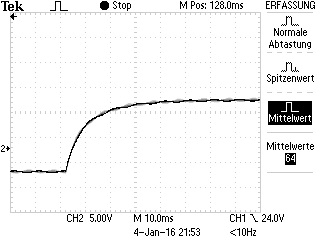
\includegraphics[width=0.7\linewidth]{data/ALL0002/F0002TEK.jpg}
    \caption{Messkurve der ansteigenden Flanke des Isotops Rubidium 87.}
    \label{fig:exp_87_raw}
    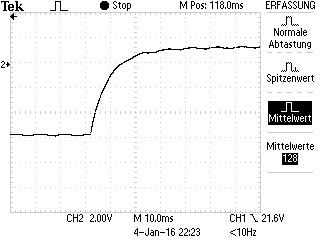
\includegraphics[width=0.7\linewidth]{data/ALL0003/F0003TEK.jpg}
    \caption{Messkurve der ansteigenden Flanke des Isotops Rubidium 85.}
    \label{fig:exp_85_raw}
\end{figure}

\begin{figure}[!h]
    \centering
    \includegraphics[width=0.7\linewidth]{build/plots/fit_E_87.pdf}
    \caption{Ansteigende Kurve der RF-Modulation des Rubidium Isotops 87.}
    \label{fig:exp_87}
    \includegraphics[width=0.7\linewidth]{build/plots/fit_L_87.pdf}
    \caption{Logarithmische Darstellung der ansteigenden Kurve der RF-Modulation des Rubidium Isotops 87. Im linearen Bereich der Funktion wurde eine lineare Regression duchgeführt.}
    \label{fig:exp_87_fit}
\end{figure}

\begin{figure}[!h]
    \centering
    \includegraphics[width=0.7\linewidth]{build/plots/fit_E_85.pdf}
    \caption{Ansteigende Kurve der RF-Modulation des Rubidium Isotops 85.}
    \label{fig:exp_85}
    \includegraphics[width=0.7\linewidth]{build/plots/fit_L_85.pdf}
    \caption{Logarithmische Darstellung der ansteigenden Kurve der RF-Modulation des Rubidium Isotops 85. Im linearen Bereich der Funktion wurde eine lineare Regression duchgeführt.}
    \label{fig:exp_85_fit}
\end{figure}

\FloatBarrier
\subsubsection{Perioden der RF-Modulation} % (fold)
\label{ssub:perioden_der_rf_modulation}

Die untersuchung der Perioden der RF-Modulation erfolgt an der absteigenden Flanke der RF-Modulation.
Die gemessenen Zeiten und die daraus ermittelten Perioden sind in den Tabellen \ref{tab:T_87_raw} und \ref{tab:T_85_raw} dargestellt.
Wird nun die Periode $T$ gegen die Spannung $V$ aufgetragen, lässt sich die Funktion mithilfe einer Regression der Form $e(U)=a_\text{87} + b_\text{87}/(U - c_\text{87})$ und $f(U)=a_\text{85} + b_\text{85}/(U - c_\text{85})$ ermitteln.
Es ergeben sich somit die Koeffizienten zu
\begin{align*}
    a_\text{87} &= \input{build/tex/i_fit_T_a_87.tex} \,,\\
    b_\text{87} &= \input{build/tex/i_fit_T_b_87.tex} \,,\\
    c_\text{87} &= \input{build/tex/i_fit_T_c_87.tex} \,,\\
    a_\text{85} &= \input{build/tex/i_fit_T_a_85.tex} \,,\\
    b_\text{85} &= \input{build/tex/i_fit_T_b_85.tex} \,,\\
    c_\text{85} &= \input{build/tex/i_fit_T_c_85.tex} \,.
\end{align*}
Das Ergebnis ist in den Graphiken \ref{fig:T_87} und \ref{fig:T_85} aufgetragen.
Eine Berechnung des Quotienten $b_\text{87}/b_\text{85}$ ergibt $b_\text{87}/b_\text{85} = \input{build/tex/i_fit_T_quot.tex}$.

\begin{table}[!h]
    \centering
    \caption{Aufgenommene Daten, welche zur Berechnung der Perioden der RF-Modulation des Isotops Rubidium 87 genutzt wurden und die resultierende Periode.}
    \input{build/tex/t_87.tex}
    \label{tab:T_87_raw}
    \\
    \caption{Aufgenommene Daten, welche zur Berechnung der Perioden der RF-Modulation des Isotops Rubidium 85 genutzt wurden und die resultierende Periode.}
    \input{build/tex/t_85.tex}
    \label{tab:T_85_raw}
\end{table}

\begin{figure}[!h]
    \centering
    \includegraphics[width=0.7\linewidth]{build/plots/fit_T_85.pdf}
    \caption{Periode aufgetragen gegen die Spannung zur Berechnung der Funktion $e(U)$.}
    \label{fig:T_85}
    \includegraphics[width=0.7\linewidth]{build/plots/fit_T_87.pdf}
    \caption{Periode aufgetragen gegen die Spannung zur Berechnung der Funktion $f(U)$.}
    \label{fig:T_87}
\end{figure}

\FloatBarrier
\section{Diskussion} % (fold)
\label{sec:diskussion}

Mithilfe dieses Versuchsaufbau lassen sich gute Ergebnisse erzielen und er ist somit zur Berechnung der gesuchten größen geeignet.
Es war ohne Probleme möglich die Isotope mithilfe des Magnetfeldes zu separieren.

Die Untersuchung des Isotopenverhältnisses in der Probe ergab für Rubidium 87 $\SI{35.3 \pm 2.2}{\percent}$ und für Rubidium 85 $\SI{64.7 \pm 2.2}{\percent}$.
Es is somit mehr Rubidium 87 vorhanden als in dem natürlichen Isotopenverhältnis von Rubidium 87 $\SI{27.83(2)}{\percent}$ \cite{spin_rubidium} und Rubidium 85 $\SI{72.17(2)}{\percent}$ \cite{spin_rubidium}.

Der gemessene Wert für das lokale Erdmagnetfeld in der Horizontalkomponente $B_\text{Hor} = \SI{18.2 \pm 0.4}{\micro\tesla}$ weichte um etwa $\SI{3}{\percent}$ vom theoretischen Wert $B_\text{Theo, Hor} = \SI{18.8}{\micro\tesla}$ \cite{earth_magnetism} ab.
In der Vertikalkomponente weicht der bestimmte Wert $B_\text{Vert} = \SI{39.84 \pm 0.08}{\micro\tesla}$ hingegen um etwa $\SI{14}{\percent}$ vom theoretischen Wert $B_\text{Theo, Vert} = \SI{45.5}{\micro\tesla}$ \cite{earth_magnetism} ab.

Aus den errechneten Landé-Faktoren war es möglich die Kernspins hinreichend genau zu bestimmen.
So weicht der errechnete Wert für Rubidium 85 $\text{I}_\text{85} = \input{build/tex/c_I_85.tex}$ um etwa $\SI{1}{\percent}$ vom Literaturwert $\SI{2.5}{}$ \cite{spin_rubidium} ab.
Für Rubidium 87 ergibt sich $\text{I}_\text{87} = \input{build/tex/c_I_87.tex}$ und somit eine Abweichung von etwa $\SI{0.3}{\percent}$ vom Literaturwert $\SI{1.5}{}$ \cite{spin_rubidium}.

Bei der Abschätzung des quadratischen Zeeman-Effekts ergab sich, dass dieser mindestens drei Größenordnungen kleiner ist als der Term erster Ordnung und dieser ist bei der Berechnung somit vernachlässigbar klein.

Bei der Untersuchung der Perioden der RF-Modulation errechnete sich ein Wert von $b_\text{87}/b_\text{85} = \input{build/tex/i_fit_T_quot.tex}$, welcher um etwa $\SI{11}{\percent}$ vom Theoriewert $\SI{1.5}{}$ abweicht \cite{V21}.
